\section{Results for the rings of 6-poles}\label{sec:results6}

\subsection{Conducted sets of the 6-poles}\label{sec:conducted}

\begin{proposition}[\claim{MV}]\label{prop:core}
Let $H$ be the Petersen graph, the flower snark $J_5$ or $J_7$, or the dodecahedron. Every 6-pole
$H - u - w$ ($u$, $w$ non-adjacent, connectors at $u$ and at $w$), and, for $H \ne J_7$, every
6-pole $H - e_1 - e_2 - e_3$ ($e_1, e_2, e_3$ pairwise disjoint, any split of the six ends) conducts
$\Oz$, $\OEc$ and $\ODtwo$; the set $\{\Oz, \OEc, \ODtwo\}$
itself is conducted by $\PG - u - w$.
\end{proposition}

\begin{proof}
One formula for each 6-pole up to automorphisms of $H$, each split and each orbit, with the class of
the first connector fixed to a representative of the orbit (\nSplits{} splits, \nFormulasSix{} formulas; Table~\ref{tab:splits}). The
satisfiable ones give maps accepted by the checker, the others are refuted with DRAT proofs
accepted by \texttt{drat-trim}; none of the four graphs has a cycle-separating cut of at most four
edges.
\end{proof}

\begin{table}[t]\centering\footnotesize
\setlength{\tabcolsep}{2.6pt}
\begin{tabular}{lrrrrrrrr}
\toprule
conducted set & $\PG$ (a) & $\PG$ (b) & dodecahedron (a) & dodecahedron (b) & $J_5$ (a) & $J_5$ (b) & $J_7$ (a) & total \\
\midrule
$\{\Oz,\OEc,\ODtwo\}$ & 1 & 1 & . & 3 & 6 & 7 & 8 & 26 \\
$\{\Oz,\OEc,\ODthree,\ODtwo\}$ & . & 16 & . & 68 & 3 & 523 & 5 & 615 \\
$\{\Oz,\OEc,\ODtwo,\OTone\}$ & . & . & . & . & 1 & 1 & 1 & 3 \\
$\{\Oz,\OEc,\ODtwo,\OTtwo\}$ & . & 3 & . & 2 & 3 & 4 & 5 & 17 \\
$\{\Oz,\OEc,\ODthree,\ODtwo,\OTone\}$ & . & 4 & 2 & 10 & . & 93 & . & 109 \\
$\{\Oz,\OEc,\ODthree,\ODtwo,\OTtwo\}$ & . & 11 & 2 & 180 & . & 753 & . & 946 \\
$\{\Oz,\OEc,\ODthree,\ODtwo,\OTone,\OTtwo\}$ & . & 5 & . & 37 & 1 & 129 & 2 & 174 \\
\midrule
6-poles (splits) & 1 & 4 (40) & 4 & 30 (300) & 14 & 151 (1510) & 21 & 1{,}890 \\
formulas & 6 & 240 & 24 & 1{,}800 & 84 & 9{,}060 & 126 & 11{,}340 \\
\bottomrule
\end{tabular}
\caption{Conducted sets of the 1{,}890 six-pole splits measured by computation EXP-013 (\texttt{conduct-*.json}): the number of splits of each source and shape (a: $H - u - w$; b: $H - e_1 - e_2 - e_3$) whose set of conducted orbits is the set in the first column. A dot is zero. Every split conducts $\Oz$, $\OEc$ and $\ODtwo$; the smallest set that occurs is that core, from $\PG - u - w$. All 11{,}340 formulas are decided, each answer checked.}\label{tab:splits}
\end{table}


Table~\ref{tab:splits} and Figure~\ref{fig:conducted} show how the conducted sets are distributed. Every one of the
\nSplits{} measured splits conducts $\Oz$, $\OEc$ and $\ODtwo$, and the three orbits $\ODthree$, $\OTone$, $\OTtwo$ are conducted by
subsets of them: seven distinct sets occur, from the core $\{\Oz,\OEc,\ODtwo\}$ (26 splits, among them $\PG - u - w$) to the set of all six orbits
(174 splits). The prediction that some 6-pole of a cyclically 5-edge-connected source fails to conduct $\Oz$ is refuted: the \nSplitsB{}
shape-(b) splits all conduct it. Consequently no two of these 6-poles have disjoint conducted sets, and the ring theorem of
Section~\ref{sec:rings} cannot show that a ring of them has no Petersen coloring.

\begin{figure}[t]\centering
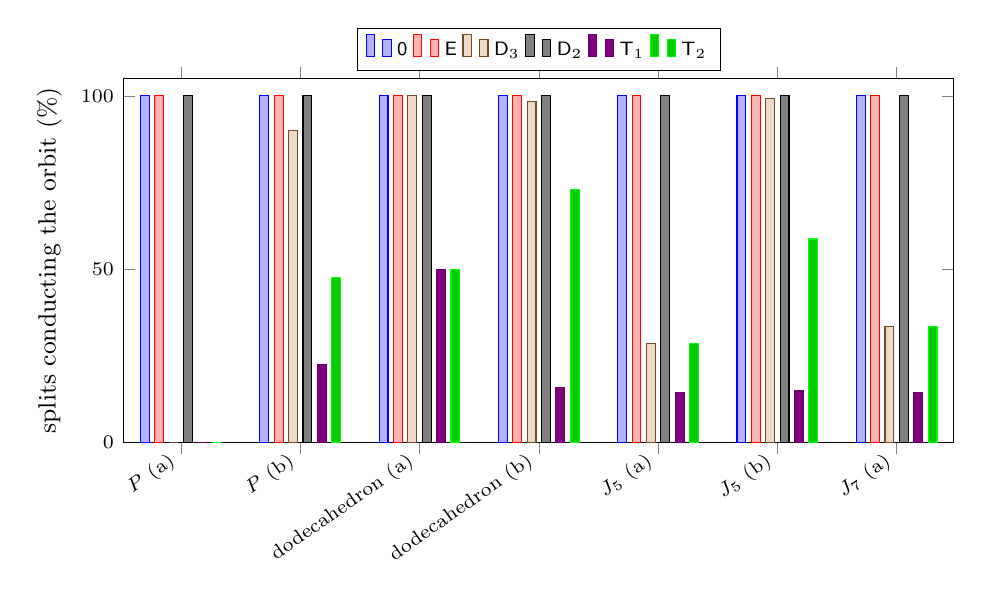
\begin{tikzpicture}
\begin{axis}[ybar,width=\textwidth,height=6.2cm,bar width=3.2pt,ymin=0,ymax=105,ylabel={splits conducting the orbit (\%)},symbolic x coords={Pa,Pb,Dodecaa,Dodecab,J5a,J5b,J7a},xtick=data,xticklabels={$P$ (a),$P$ (b),dodecahedron (a),dodecahedron (b),$J_5$ (a),$J_5$ (b),$J_7$ (a)},x tick label style={font=\scriptsize,rotate=35,anchor=east},tick label style={font=\scriptsize},label style={font=\small},legend style={font=\scriptsize,at={(0.5,1.02)},anchor=south,legend columns=6},enlarge x limits=0.08]
\addplot coordinates {(Pa,100.0) (Pb,100.0) (Dodecaa,100.0) (Dodecab,100.0) (J5a,100.0) (J5b,100.0) (J7a,100.0)};
\addplot coordinates {(Pa,100.0) (Pb,100.0) (Dodecaa,100.0) (Dodecab,100.0) (J5a,100.0) (J5b,100.0) (J7a,100.0)};
\addplot coordinates {(Pa,0.0) (Pb,90.0) (Dodecaa,100.0) (Dodecab,98.3) (J5a,28.6) (J5b,99.2) (J7a,33.3)};
\addplot coordinates {(Pa,100.0) (Pb,100.0) (Dodecaa,100.0) (Dodecab,100.0) (J5a,100.0) (J5b,100.0) (J7a,100.0)};
\addplot coordinates {(Pa,0.0) (Pb,22.5) (Dodecaa,50.0) (Dodecab,15.7) (J5a,14.3) (J5b,14.8) (J7a,14.3)};
\addplot coordinates {(Pa,0.0) (Pb,47.5) (Dodecaa,50.0) (Dodecab,73.0) (J5a,28.6) (J5b,58.7) (J7a,33.3)};
\legend{$\mathsf{0}$,$\mathsf{E}$,$\mathsf{D}_3$,$\mathsf{D}_2$,$\mathsf{T}_1$,$\mathsf{T}_2$}
\end{axis}
\end{tikzpicture}

\caption{Share of the splits of each source and shape that conduct each of the six orbits (computation EXP-013, \texttt{conduct-*.json}): the orbits
$\mathsf{0}$, $\mathsf{E}$ and $\mathsf{D}_2$ are conducted by every split (100\,\%), the others by a varying share.}\label{fig:conducted}
\end{figure}

\begin{table}[t]\centering\small
\begin{tabular}{lrr}
\toprule
conducted set & 6-poles $\Gfty - u - w$ & share \\
\midrule
$\{\OEc,\ODthree,\ODtwo\}$ & 105 & 49.5\,\% \\
$\{\OEc,\ODthree,\ODtwo,\OTtwo\}$ & 47 & 22.2\,\% \\
$\{\OEc,\ODtwo\}$ & 32 & 15.1\,\% \\
$\{\OEc\}$ & 22 & 10.4\,\% \\
$\{\OEc,\ODthree\}$ & 5 & 2.4\,\% \\
$\{\OEc,\ODtwo,\OTtwo\}$ & 1 & 0.5\,\% \\
\midrule
$\Oz$ conducted by & 0 of 212 & \\
$\OEc$ conducted by & 212 of 212 & \\
$\OTone$ conducted by & 0 of 212 & \\
\bottomrule
\end{tabular}
\caption{Charge spectrum of the 212 orbits of 6-poles $\Gfty - u - w$ ($u$, $w$ non-adjacent; computation EXP-013, \texttt{conduct-G52-a.json}, 1,272 formulas, slowest formula 106.6 s). No pair of non-adjacent vertices carries class $\Oz$, as the restoration argument requires; every pair can carry class $\OEc$; no pair carries the all-ones class.}\label{tab:g52}
\end{table}


The charge spectrum of the 52-vertex counterexample differs in kind (Table~\ref{tab:g52}). Of its 212 orbits of 6-poles $\Gfty - u - w$ none
conducts $\Oz$, which is the restoration argument of Section~\ref{sec:theory6} confirmed by 212 refutations, every pair conducts $\OEc$, and none conducts
$\OTone$. So every critical pair of $\Gfty$ can carry a charge of the class of a single edge, 22 of the 212 pair orbits carry only such charges, and no
pair carries the all-ones class.

\subsection{Sector matrices of the 81 blocks}\label{sec:blocks}

\begin{table}[t]\centering\footnotesize
\setlength{\tabcolsep}{3pt}
\begin{tabular}{lrrrrrr}
\toprule
family & blocks & vertices & time, max (s) & time, mean (s) & entries, mean & re-checked \\
\midrule
claw $Y$ & 1 & 4 & 0.2 & 0.2 & 432 & 1 of 1 \\
superedge $S$ & 1 & 8 & 1.1 & 1.1 & 424 & 1 of 1 \\
$\PG$, shape b & 40 & 10 & 1.5 & 0.5 & 881 & 38 of 40 \\
dodecahedron, shape a & 4 & 18 & 5.8 & 4.3 & 1{,}208 & 3 of 4 \\
$J_5$, shape a & 14 & 18 & 16.3 & 11.3 & 1{,}547 & 3 of 14 \\
$J_7$, shape a & 21 & 26 & 202.3 & 83.3 & 2{,}706 & 0 of 21 \\
\midrule
all & 81 & & 202.3 & 24.0 $\pm$ 41.0 & & 46 of 81 \\
\bottomrule
\end{tabular}
\caption{The 81 blocks whose six sector matrices were computed (computation EXP-014, \texttt{blocks.json}, \texttt{block-recheck.json}): per family the number of blocks, the vertices of each, the maximal and mean computation time, the mean number of nonzero matrix entries over the six sectors, and the number recomputed with the second encoding and second solver. The claw and the superedge were also recomputed by exhaustive enumeration of maps. Not reached: 2 of the 40 $\PG$ blocks, 1 of the 4 dodecahedron blocks, 11 of the 14 $J_5$ blocks and all 21 $J_7$ blocks. The $\pm$ value is the sample standard deviation of the 81 times.}\label{tab:blocks}
\end{table}


The sector matrices of all 81 blocks were computed by Algorithm~\ref{alg:sector} (Table~\ref{tab:blocks}). The nonempty sectors of every block
equal the conducted orbits that computation EXP-013 measured independently for the same 6-pole and split, for example for all 14 shape-(a) blocks of $J_5$. The claw $Y$
conducts $\{\Oz, \OEc, \ODthree, \ODtwo, \OTone\}$ and the superedge $S = \PG - u - w$ conducts $\{\Oz, \OEc, \ODtwo\}$, with \nSuperedgeZero, \nSuperedgeE{} and
\nSuperedgeDtwo{} entries in those sectors. The sector-$\Oz$ matrix of the superedge has exactly two entries in each row: a star at $u$ extends in exactly two ways,
the two automorphisms of $\PG$ that fix $u$ and its three neighbors. The re-check against the second encoding reached 46 of the 81 blocks
and found no difference; the 35 not reached are named by family in Table~\ref{tab:blocks}.

\subsection{Closures and the ring theorems}\label{sec:closures}

\begin{table}[t]\centering\footnotesize
\setlength{\tabcolsep}{3.5pt}
\begin{tabular}{lrrrrrrrrl}
\toprule
 & & \multicolumn{3}{c}{exact closure} & \multicolumn{3}{c}{antichain certificate} & & \\
\cmidrule(lr){3-5}\cmidrule(lr){6-8}
family & gen. & elements & word & s & elements & word & s & zero trace & status \\
\midrule
$F_1 = \{Y\}$ & 6 & 30 & 6 & 0.0 & 12 & 3 & 0.3 & 0 & closed, checked \\
$F_2 = \{S\}$ & 6 & 19{,}005 & 12 & 27.1 & 276 & 5 & 5.0 & 0 & closed, checked \\
$F_3 = \{Y, S\}$ & 12 & 116{,}463 & 13 & 344.6 & 2{,}454 & 6 & 349.4 & 0 & closed, checked \\
$F_4$ (40 blocks of $\PG$) & 336 & 200{,}070 & 3 & 93.4 & n/a & n/a & 3{,}600 & none found & undecided \\
$F_5$ (all 81 blocks) & 684 & n/a & n/a & n/a & n/a & n/a & 3{,}600 & none found & undecided \\
\bottomrule
\end{tabular}
\caption{The closures of the block families $F_1$ to $F_5$ (computation EXP-014, \texttt{closure-F*.json}, \texttt{certificate-check-antichain.json}): the distinct generators, the elements of the exact closure of products of at least two generators with the longest new word and time, and the antichain certificate with its longest word and time. The exact closure of $F_4$ stopped at the cap of 200{,}000 elements (200{,}070 stored, word length 3) with no zero-trace element among them. The antichain closures of $F_4$ and $F_5$ reached their one-hour limit inside the products of two generators; the generators and limit of $F_5$ are those of the experiment record, which keeps no artifact for it. Both are undecided.}\label{tab:closures}
\end{table}


\begin{figure}[t]\centering
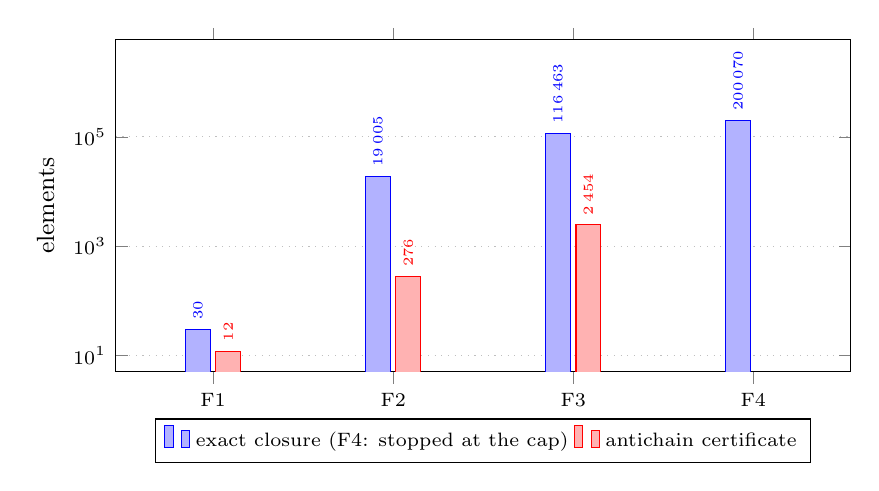
\begin{tikzpicture}
\begin{axis}[ybar,width=0.9\textwidth,height=5.8cm,ymode=log,bar width=9pt,ymin=5,ymax=6000000,symbolic x coords={F1,F2,F3,F4},xtick=data,ylabel={elements},tick label style={font=\scriptsize},label style={font=\small},legend style={font=\scriptsize,at={(0.5,-0.14)},anchor=north,legend columns=2},enlarge x limits=0.18,ymajorgrids=true,grid style={dotted},nodes near coords,nodes near coords style={font=\tiny,rotate=90,anchor=west,/pgf/number format/.cd,fixed,precision=0,1000 sep={\,}},point meta=rawy]
\addplot coordinates {(F1,30) (F2,19005) (F3,116463) (F4,200070)};
\addplot coordinates {(F1,12) (F2,276) (F3,2454)};
\legend{exact closure (F4: stopped at the cap),antichain certificate}
\end{axis}
\end{tikzpicture}

\caption{Sizes of the exact closure and of the antichain certificate of the four families that were attempted (computation EXP-014, \texttt{closure-F*.json}, logarithmic scale);
the bar of $F_4$ is the number of elements stored when the closure stopped at the cap of 200{,}000, not a closure size.}\label{fig:closures}
\end{figure}

\begin{table}[t]\centering\small
\begin{tabular}{llrrrrrrr}
\toprule
family & closure & elements & $\Oz$ & $\OEc$ & $\ODthree$ & $\ODtwo$ & $\OTone$ & $\OTtwo$ \\
\midrule
$F_1$ & exact & 30 & 15 & 18 & 7 & 9 & 13 & 0 \\
$F_1$ & certificate & 12 & 6 & 6 & 1 & 3 & 4 & 0 \\
$F_2$ & exact & 19{,}005 & 11{,}230 & 19{,}005 & 0 & 3 & 0 & 0 \\
$F_2$ & certificate & 276 & 52 & 276 & 0 & 1 & 0 & 0 \\
$F_3$ & exact & 116{,}463 & 64{,}854 & 116{,}451 & 7 & 529 & 13 & 0 \\
$F_3$ & certificate & 2{,}454 & 595 & 2{,}448 & 1 & 31 & 4 & 0 \\
$F_4$ & exact, stopped at the cap & 200{,}070 & 192{,}194 & 200{,}035 & 5{,}998 & 176{,}996 & 372 & 345 \\
\bottomrule
\end{tabular}
\caption{Number of elements of each closure with a nonzero diagonal in each of the six sectors (computation EXP-014, \texttt{closure-F*.json}). In $F_2$ the sector $\OEc$ has a nonzero diagonal for every element, the sector $\Oz$ for 11{,}230 elements and $\ODtwo$ for 3; the sectors $\ODthree$, $\OTone$ and $\OTtwo$ have none. The claw family $F_1$ has no element in $\OTtwo$. The row of $F_4$ counts the elements stored when the closure stopped.}\label{tab:sectors}
\end{table}


Table~\ref{tab:closures} and Figure~\ref{fig:closures} give the closures. For $F_1$, $F_2$ and $F_3$ the closure is complete, has no zero-trace element, and
the antichain certificate is much smaller: \nCertFtwo{} elements for the \nElemFtwo{} of $F_2$ and \nCertFthree{} for the \nElemFthree{} of $F_3$, with the longest new word shortening
from 12 to 5 and from 13 to 6. The family $F_4$ is undecided: its exact closure of products of at least two of the 336 generators stopped at the cap with \nElemFfour{} elements at word length 3,
and the antichain closures of $F_4$ and of $F_5$ reached the one-hour limit inside the products of two generators; no zero-trace element was found among the products computed.
Table~\ref{tab:sectors} shows in which sectors the closure elements are colorable.

\begin{theorem}[\claim{MV}]\label{thm:ringsY}
Every ring of at least two blocks, each a claw or a Petersen superedge in either orientation, joined
through arbitrary bijections, has a Petersen coloring. A ring of Petersen superedges always has one
whose joining edges carry classes of the orbit $\OEc$.
\end{theorem}

\begin{proof}
The sector matrices of $Y$ and $S$ were computed by Algorithm~\ref{alg:sector}, each model accepted by the checker, and recomputed by exhaustive
enumeration of maps and by a second encoding with a second solver, with identical results. The set
of all products of at least two generators was closed exhaustively for $\{Y\}$, $\{S\}$ and
$\{Y, S\}$: it has $\nElemFone$, $\nElemFtwo$ and $\nElemFthree$ elements, all with a nonzero diagonal; for
$\{S\}$ every element has a nonzero diagonal in the sector $\OEc$. Certificates in the sense of
Corollary~\ref{cor:semigroup}, kept minimal under containment (Algorithm~\ref{alg:closure}), have $\nCertFone$, $\nCertFtwo$ and $\nCertFthree$
elements and were re-verified by Algorithm~\ref{alg:check}, a separate program with a different matrix product. The ring statements follow from Corollary~\ref{cor:semigroup}.
\end{proof}

\begin{corollary}[flower snarks, \claim{MV}, \claim{D}]\label{cor:flower}
For every odd $k \ge 5$, every Petersen coloring of $J_k$ maps the three edges joining two
consecutive claws onto an antipodal triple of $\PG$.
\end{corollary}

\begin{proof}
The products $(Y\,\mathrm{id})^{k-1}(Y\,\tau)$ are periodic in $k$ from $k = 5$ with period 2,
and for odd $k$ only the sector $\OTone$ has a nonzero diagonal (for even $k$ only
$\OEc$). By conduction all junctions of a coloring carry one class, which is therefore
$\OTone$, and the 30 ordered triples of class $\OTone$ are the orderings of the five
antipodal triples. The vanishing of the other diagonals rests on the completeness of the matrix of $Y$
(Lemma~\ref{lem:soundness}), which was recomputed by exhaustive enumeration and by a second encoding. For $k = 5, 7, 9$ the sector traces of the
explicit rings, rebuilt from claw words and isomorphic to the flower snarks, are $\{\OTone\}$ in all three cases (Section~\ref{sec:crosscheck}).
\end{proof}

\begin{remark}[the case $k=3$, \claim{C}]\label{rem:kthree}
The ring $(Y\,\mathrm{id})^{2}(Y\,\tau)$ is a product of three generators, hence an element of the closure of $F_1$, and by Theorem~\ref{thm:ringsY} its diagonal is nonzero in some
sector. The periodicity argument of Corollary~\ref{cor:flower} starts at $k = 5$, and the stored artifacts do not record the sector of the product for
$k = 3$ or $k = 4$ (the sector matrices themselves are kept outside the repository). Whether the three edges between consecutive claws of $J_3$ are forced onto an
antipodal triple is therefore not claimed.
\end{remark}

H\"agglund and Steffen showed that flower snarks have Petersen colorings~\cite{HS2014};
Corollary~\ref{cor:flower} describes all of them at the junctions.

\begin{proposition}[\claim{MV}, \claim{D}]\label{prop:superedgerings}
Let $S^t$ be the ring of $t$ Petersen superedges with the identity at every junction.
\begin{enumerate}
\item[\textup{(a)}] For $t \ge 3$, $S^t$ is a simple cubic graph, and it is 3-edge-colorable if and
only if $t$ is even.
\item[\textup{(b)}] For $t \ge 5$, $S^t$ has girth 5 and is cyclically 5-edge-connected.
\end{enumerate}
So for every odd $t \ge 5$, $S^t$ is a cyclically 5-edge-connected snark of girth 5 on $8t$ vertices,
and by Theorem~\ref{thm:ringsY} it has a Petersen coloring.
\end{proposition}

\begin{proof}
(a) The same reduction applies to 3-edge-colorings, with the 27 color triples of a connector as
states: the boundary relation of $S$, enumerated exhaustively, has powers of period 2, and the odd
powers have a zero diagonal. (b) An exhaustive search finds no cycle-separating cut with at most
four edges in $S^5$, whose girth is 5. $\PG - u - w$ is connected, and restoring $u$ and $w$ gives
$\PG$, which is 3-edge-connected, so a ring carries six edge-disjoint paths between any two blocks.
The argument of Lemma~\ref{lem:c4ec}, with cuts of at most four edges, at most four split blocks
and runs of at most four consecutive blocks (all of which occur in $S^5$), shows that $S^t$ has no
cycle-separating cut with at most four edges for $t \ge 5$, and a cycle of length at most four would
lie in such a run.
\end{proof}

The probes on superedge rings with the same junction permutation at every junction (3 to 8 superedges, descriptive measurements with exhaustive searches) add that the ring is a snark
exactly for odd $t$ with the identity or one transposition ($t = 3, 5, 7$ checked, girth 3 at $t = 3$), that every other uniform ring with $t$ from 2 to 8 is 3-edge-colorable,
and that the rings of three and four superedges with a non-identity junction are cyclically 5-edge-connected of girth 5 as well, though 3-edge-colorable.

\subsection{Cross-check against the explicit graphs}\label{sec:crosscheck}

\begin{table}[t]\centering\small
\begin{tabular}{lrr}
\toprule
sectors with a nonzero diagonal & random rings & share \\
\midrule
$\{\Oz,\OEc\}$ & 126 & 63.0\,\% \\
$\{\Oz,\OEc,\ODtwo\}$ & 47 & 23.5\,\% \\
$\{\OEc\}$ & 19 & 9.5\,\% \\
$\{\Oz,\OEc,\ODthree\}$ & 2 & 1.0\,\% \\
$\{\Oz,\OEc,\ODthree,\ODtwo\}$ & 2 & 1.0\,\% \\
$\{\OEc,\ODtwo\}$ & 2 & 1.0\,\% \\
$\{\Oz\}$ & 1 & 0.5\,\% \\
$\{\Oz,\OEc,\OTtwo\}$ & 1 & 0.5\,\% \\
\midrule
$J_5$, $J_7$, $J_9$ (rebuilt from claw words) & \multicolumn{2}{r}{$\{\OTone\}$ in each} \\
order of the random rings & \multicolumn{2}{r}{mean $62.6 \pm 25.4$, range 18 to 132} \\
\bottomrule
\end{tabular}
\caption{Sector traces of the 200 random rings of the cross-check (computation EXP-014, \texttt{crosscheck.json}): for each set of sectors, the number of rings whose product of sector matrices has a nonzero diagonal exactly in those sectors. In every case the solver also found a Petersen coloring. The $\pm$ value is the sample standard deviation of the orders.}\label{tab:cross}
\end{table}


The sector traces were compared with CaDiCaL on the explicit cubic graph for \nCrossRings{} rings: the flower snarks $J_5$, $J_7$, $J_9$ rebuilt from claw words, and \nCrossRandom{} random words of
length 2 to 6 over all 81 blocks, with orders \nCrossOrderMin{} to \nCrossOrderMax{} (Table~\ref{tab:cross}). The two answers agree in all
\nCrossRings{} cases, and all \nCrossRings{} rings are Petersen colorable. This comparison therefore tests one direction only, which Section~\ref{sec:ablation} analyses. The random words have lengths from 2 to 6 (\nCrossLenTwo{} of length 2
and \nCrossLenSix{} of length 6), and \nCrossTraceE{} of the 200 rings have a nonzero diagonal exactly in the sectors $\{\Oz,\OEc\}$; the sector $\OEc$ carries a coloring of every random ring but one, and no random ring has a
zero trace.
